\section{Bifurcation de fold-hopf}

Pour qu'un système soit qualifié d'élément de bascule, il doit être possible d'y identifier un paramètre de forçage $\phi$ pour lequel il existe une certaine valeur critique $\phi_c$ telle qu'une petite perturbation $\delta \phi$ induise un changement qualitatif dans la structure du système.
Cette bifurcation apparaît dans un système d'équations différentielles ordinaires (EDOs) $f: \Omega \subseteq \R^n \rightarrow \R^n$ constitué à la fois d'une EDO sur la droite ($\Omega = \R$) et d'un système d'EDOs dans le plan ($\Omega = \R^2$). De ce premier système surgissent deux bifurcations de type \emph{"fold"} tandis que du second système surgit une bifurcation de type \emph{"hopf"}.

Nous considérerons le système suivant,
\begin{equation} \label{eq:fold-hopf}
  \begin{cases}
    \dot{x} = a_1x^3 + a_2x + \phi \\
    \dot{y} = b_1z + b_2(\gamma(x) - (y^2 + z^2))y \\
    \dot{z} = c_1y + c_2(\gamma(x) - (y^2 + z^2))z
  \end{cases}
\end{equation}
où $\phi$ est un paramètre de forçage et $\gamma(x) = \gamma_1 + \gamma_2 x$, $\gamma_1$, $\gamma_2 \in \R$ est un paramètre de couplage linéaire.
Nous appellerons $\dot{x}$ le \textbf{système primaire} et l'ensemble $\dot{y}$ et $\dot{z}$ le \textbf{système secondaire}.

Alors que nous nous approchons de la valeur critique de la bifurcation que nous noterons $\phi_{c}$, une petite perturbation du paramètre $\phi$ suffit pour passer la bifurcation et modifier considérablement le comportement qualitatif du système. Dans le langage des systèmes dynamiques on dit qu'il y a création, suppression d'équilibres voir modification dans la nature de ces équilibres. Toutefois, dans la définition des points de bascules, il en existe certains qui sont réversibles et qui ne sont donc pas dû à des bifurcations (\cite{lenton_tipping_2008}). Nous ne considérerons pas ces derniers dans cet article.

\subsection{Bifurcation fold} \label{sec:fold}

\begin{figure*}[H]
  \centering
  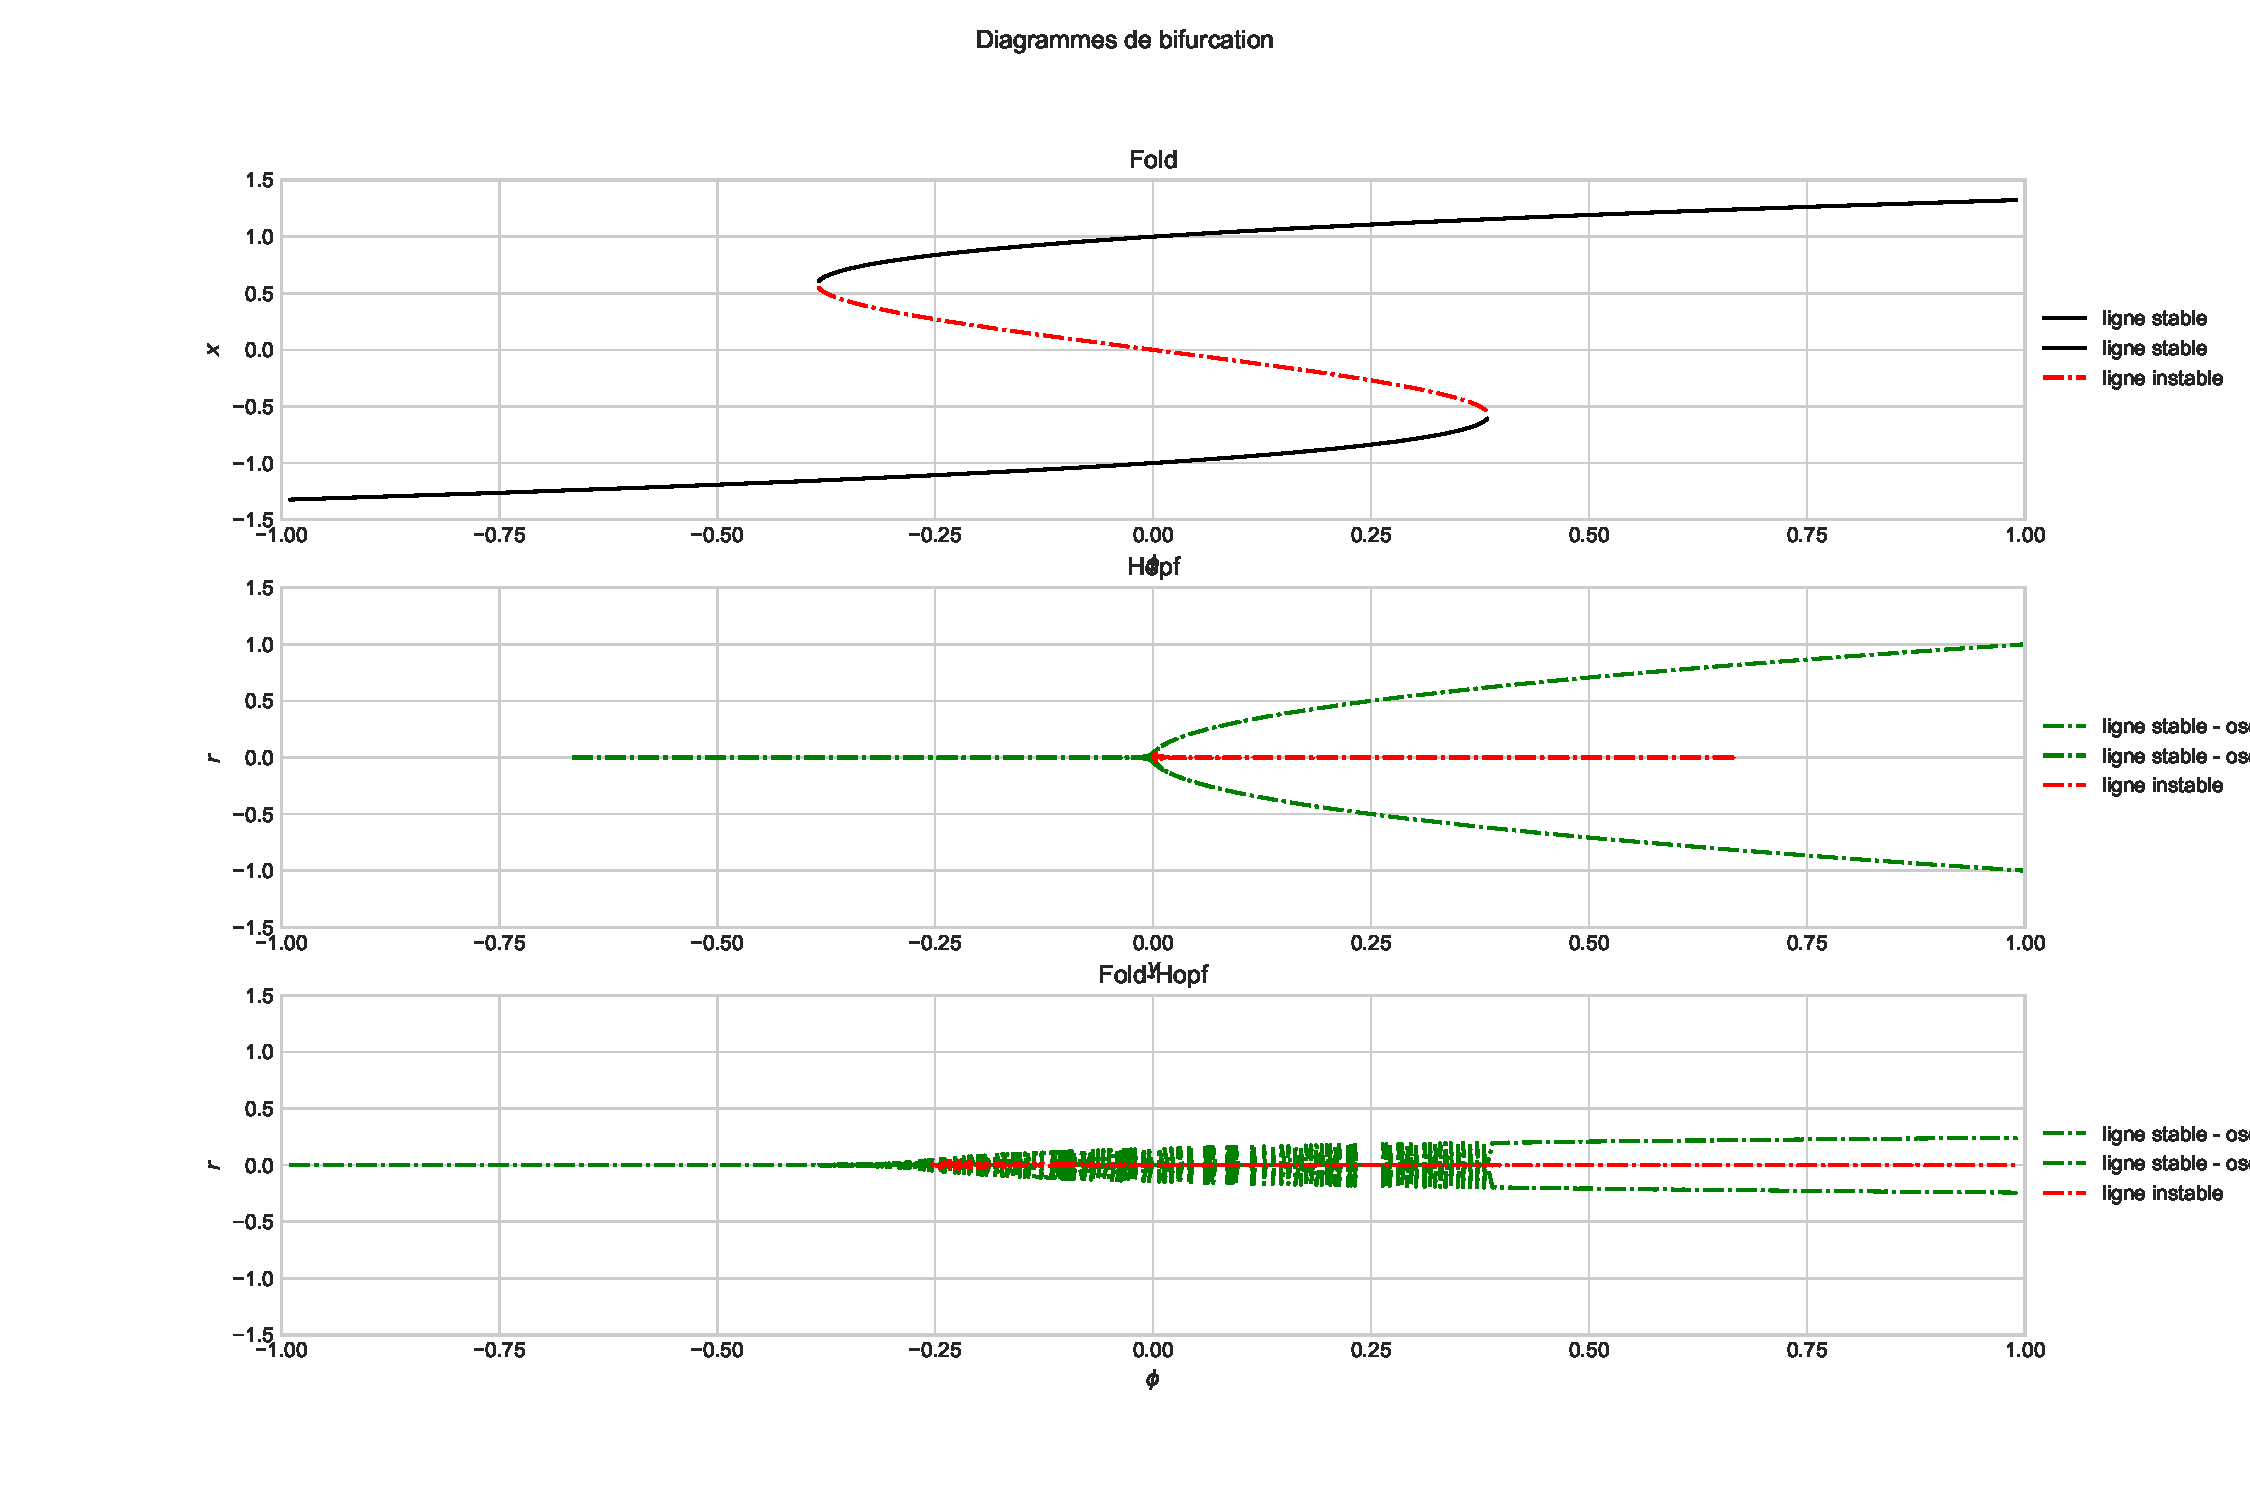
\includegraphics{figures/bifurcations.pdf}
  \caption{(a) Système primaire vs forçage $\phi$. (b) Système secondaire vs couplage $\gamma$. (c) Système secondaire vs forçage $\phi$. Les lignes noires correspondent aux équilibres stables tandis que les lignes rouges en traits pointillés correspondent aux équilibres instables. Les lignes vertes en traits pointillés correspondent à un équilibre stable présentant un régime oscillatoire. Les points rouges sont les points de bascule de la bifurcation fold tandis que les points oranges sont les points de bascule de la bifurcation de hopf.}
  \label{fig:bifurcations}
\end{figure*}

Considérons le système primaire,
\begin{equation} \label{eq:fold}
  \dot{x}(t) = a_1 x^3 + a_2 x + \phi \equiv f_{\phi}(x),  \quad a_1, a_2 \in \R
\end{equation}
Cette équation fait apparaître une bifurcation fork qui est une combinaison de 2 bifurcations points de selle (fold). Une bifurcation point de selle consiste en l'apparition de 2 équilibres, un stable et un instable lorsqu'on atteint une certaine valeur de $\phi$. La bifurcation fork consiste en l'apparition de 3 équilibres, 2 stables et 1 instable lorsque $\phi$ se trouve dans un certain intervalle induisant alors une bistabilité.

Cette bifurcation a la particularité de présenter un phénomène dit \emph{d'hystérésis} c'est à dire que le système se comporte à la fois selon la valeur courante du paramètre de forçage mais également selon son historique.

On peut retrouver l'intervalle de bistabilité en cherchant les équilibres du système. Le système dispose d'un ou plusieurs points d'équilibres en $x = x_0$ lorsque $f_{\phi}(x_0) = 0$. On peut voir cette EDO comme la somme de 2 courbes, $f_1(x) = a_1 x^3$ et $f_2(x) = - (a_2x + \phi_c)$. Les équilibres du système correspondent aux points d'intersection de $f_1$ et $f_2$. Si l'on trace ces 2 fonctions, on remarque la création de 2 équilibres lorsque la droite $f_2$ est tangente à la fonction cubique $f_1$. On peut de par cette observation facilement repérer nos points d'équilibres
\begin{equation}
  f_{\phi_c}'(x_0) = 0 \implies x_0 = \pm \sqrt{-\frac{a_2}{3a_1}}
\end{equation}

L'analyse graphique nous montre qu'il s'agit de 2 équilibres stables. Il existe également un équilibre instable situé entre ces 2 derniers.
Si l'on injecte cette valeur de $x_0$ dans l'équation pour la condition d'équilibre du système $f_{\phi}(x_0) = 0$, on trouve après un peu d'algèbre l'intervalle de bistabilité où se trouve les 3 équilibres du système,
\begin{equation} \label{eq:phi_c-range}
  |\phi_c| < \sqrt{\frac{-4(a_2)^3}{27a_1}}
\end{equation}
où $a_1 < 0 < a_2$ ou $a_1 > 0 > a_2$.

Pour des valeurs de paramètres cités dans le \autoref{tab:parameters} cet intervalle vaut $]-0.38, 0.38[$.

% TODO: trouver mathématiquement l'équilibre instable x_0^(instable)

On peut mieux se rendre compte de la dynamique du système en traçant son diagramme de bifurcation (\autoref{fig:bifurcations}a).
Lorsqu'on approche $\phi_c$ par des valeurs $\phi < \phi_c$, le système est dans un état stable. Une fois que l'on atteint $\phi_c$ (dans le système climatique il pourrait s'agit d'une température critique, une concentration de CO2 critique,\dots), le système est attiré vers un nouvel état stable (branche supérieur de la \autoref{fig:bifurcations}a). Si le paramètre de forçage continue d'augmenter, le système reste stable. Par contre si un quelconque phénomène arrivait à baisser la valeur de $\phi$ jusqu'à la valeur $-\phi_c$, le système repasserait dans l'état stable initial. On voit bien que diminuer la valeur du paramètre de forçage une fois la transition critique faite ne fait pas directement repasser le système dans son état initial. Il s'agit bien là d'un phénomène d'hystérésis. Un raisonnement analogue peut être fait si l'on approche $-\phi_c$ par des valeurs $\phi > -\phi_c$. Toutefois, entre ces 2 branches stables existe une branche instable. Dès lors, lorsque la valeur du paramètre de forçage se trouve dans l'intervalle critique, le système se verra dans un des 2 états stables dépendant des conditions initiales (les solutions du systèmes convergeront vers la branche haute (\emph{resp. basse}) si la condition initiale $x_0$ est supérieure (\emph{resp. inférieure}) à la valeur de l'équilibre instable pour un $\phi_0$ donné appartenant à l'intervalle critique). Il est également possible que des conditions initiales fassent que le système se situe sur la courbe instable mais du fait de la nature de cet équilibre, une perturbation des conditions initiales amènerait le système à être attiré vers une des branches stables.

\subsection{Bifurcation hopf}

Considérons le système secondaire et remplaçons le paramètre de couplage $\gamma(x)$ par un paramètre de forçage $\gamma$.
\begin{equation} \label{eq:hopf}
  \begin{cases}
    \dot{y} = b_1z + b_2(\gamma - (y^2 + z^2))y \equiv f_{1,\gamma}(y,z) \\
    \dot{z} = c_1y + c_2(\gamma - (y^2 + z^2))z \equiv f_{2, \gamma}(y,z)
  \end{cases}
\end{equation}
où $b_1, b_2, c_1, c_2 \in \R$.

Les points d'équilibre sont $y = 0$ et $z = 0$ si $c_1 > 0$, $b_2c_2 < 0$ et $b_1 > 0$.
% Afin de trouver la nature de ces équilibres, on peut analyser les valeurs propres la matrice jacobienne $df$ au point d'équilibre $\vb{p} = (0, 0)$.

Sans perte de généralité, posons $b_1 = b_2 = 1$, $c_1 = -1$ et $c_2 = 1$.
% \begin{equation}
%   df(\vb{p}) =
%   \begin{pmatrix}
%     \gamma & 1 \\
%     -1 & \gamma
%   \end{pmatrix}
% \end{equation}

% %TODO: valeurs propres

Afin de mieux comprendre la façon de se comporte notre système, on peut passer en coordonnées polaires $(r, \theta)$
\begin{equation}
  \begin{cases}
    \dot{r} = \gamma r - r^3 \\
    \dot{\theta} = -1
  \end{cases}
\end{equation}

L'analyse graphique de l'équation pour $\dot{r}$ nous montre la présence d'un équilibre stable en $r = 0$ pour $\gamma < 0$ par contre lorsque $\gamma \geq 0$, l'équilibre en $r = 0$ devient instable et il apparaît un nouvel attracteur en $r = \sqrt{\gamma}$. Il y a à la fois changement dans la nature de l'équilibre en $r = 0$ et création d'un autre équilibre. La présence d'un attracteur en $r = \sqrt{\gamma}$ lorsque $\gamma \geq 0$ induit l'apparition d'un cycle limite de rayon $r = \sqrt{\gamma}$ où toutes les solutions partant en dehors de ce cycle y convergent (\autoref{fig:phase-plot}). C'est ce que nous voyons sur la figure (\ref{fig:bifurcations}b). Puisque ce cycle limite stable apparaît en une valeur de $\gamma$ supérieure à celle du point d'équilibre instable, on nomme cette bifurcation une bifurcation de hopf \emph{supercritique}.

\subsection{Bifurcation fold-hopf}

Le système que nous étudions présente un mix de ces 2 bifurcations. L'équation pour $\dot{x}$ donne lieu à 2 bifurcations fold comme nous l'avons vu à la section (\ref{sec:fold}). L'équation pour $\dot{y}$ et $\dot{z}$ est un peu différente dans le sens où nous considérons dès à présent un paramètre de couplage linéaire $\gamma(x)$ qui dépend de la première équation. Par ailleurs, nous supposerons lorsque nous élaborerons la série temporelle du système que $\phi = \phi(t)$ varie lentement en fonction du temps.

% BIFURCATION

Imaginons que l’on parte d’une valeur de $\phi < - \phi_c$. Si l’on augmente lentement le paramètre de forçage $\phi$ dans la branche basse du système primaire, une fois atteint une valeur $-\phi_c$, le système primaire entre dans son régime bistable où les solutions convergeront vers l’une des 2 branches stables du système dépendant de leurs conditions initiales. Une fois atteint $+\phi_c$, on quitte le régime bistable et toutes les solutions convergerons vers la branche stable supérieure. Une fois passé $\phi_c$, la valeur de $x$ augmente de manière conséquente comparé à son augmentation négligeable lorsque $+\phi$ se situe dans l’intervalle $]-\infty, +\phi_c[$ ce qui a pour conséquence d’augmenter significativement le paramètre de couplage $\gamma(x)$ présent dans le système secondaire. Le système génère alors par cascade un cycle limite caractérisant des solutions oscillantes où toutes les solutions convergent vers ce cycle peu importe leurs conditions initiales.

\begin{figure*}[H]
  \centering
  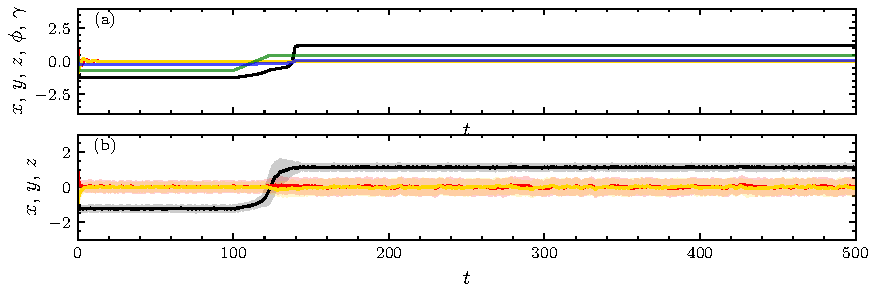
\includegraphics{figures/time-series.pdf}
  \caption{(a) Série temporelle sans bruit. (b) Série temporelle bruitée contenant un ensemble de 100 simulations avec un terme stochastique. Dans cette dernière, les lignes correspondent aux moyennes des différents états du systèmes correspondants tandis que les zones de faible opacités correspondent aux écarts-types $[\mu - \sigma, \mu + \sigma]$ des états correspondants. La ligne noire correspond au système primaire. Les lignes jaunes et rouges correspondent au système secondaire. La ligne verte est la valeur du paramètre de forçage $\phi$ et la ligne bleue est la valeur du paramètre de couplage $\gamma(x)$.}
  \label{fig:time-series}
\end{figure*}

C'est précisément ce que l'on peut remarquer sur la figure (\ref{fig:bifurcations}c). Lorsqu'on se situe dans l'intervalle $]-\infty, -\phi_c[$, le système primaire n'a qu'un seul point d'équilibre négatif ce qui a pour conséquence de laisser le système secondaire dans son état stable. Pour $\phi \in$ $]-\phi_c, +\phi_c[$, le système primaire a 3 positions d'équilibre. Pour tout $\phi$ appartenant à cet intervalle, la plus haute valeur des 3 points d'équilibre est toujours positive et en constante augmentation alors que $\phi$ augmente. Nécessairement le système secondaire ne tardera pas à passer son point de bascule à partir de valeurs de $\phi$ égales à $-\phi_c + \Delta \phi \equiv \phi_{\ast}$. Toutefois, pour les 2 autres points d'équilibres du premier système, le système secondaire restera dans son état stable. Il y a alors coexistence d'états stables et oscillatoires à partir de cette valeur de $\phi_{\ast}$. Enfin, une fois atteint l'intervalle $]\phi_c, +\infty[$, le système primaire n'a plus qu'un seul équilibre dont la valeur est telle que ce système va pousser le système secondaire uniquement dans son état où nous avons à la fois toujours 2 branches stables oscillatoires mais également une branche instable. Une représentation temporelle d'une telle cascade de bifurcations se situe sur la figure (\ref{fig:time-series}a).

Un cas où une telle bifurcation pourrait éventuellement arriver serait le cas où un effondrement de l'AMOC entraînerait un renforcement ou un affaiblissement du phénomène El-Niño (\cite{timmermann_influence_2007}). Ici, l'effondrement de l'AMOC correspond au passage de la branche basse à la branche haute dans la bifurcation fold (figure \ref{fig:bifurcations}a). Tandis que le renforcement / affaiblissement de El-Niño correspond aux 2 branches oscillatoires dans la bifurcation hopf (figure \ref{fig:bifurcations}b). Le retournement est lui forcé par le flux d'eau douce et donc ce dernier correspond au paramètre $\phi$ tandis que le couplage avec l'Océan Pacifique est assuré par les alizés\footnote{Vent régulier des régions intertropicales soufflant d'Est en Ouest de façon régulière à partir des hautes pressions subtropicales vers les basses pressions équatoriales} et correspond au paramètre $\gamma$.

% SERIES TEMPORELLES

On a vu que la transition dans le système secondaire est générée par cascade une fois que le système primaire a passé son point critique $\phi_c$. En particulier nous avons vu que la transition de ce dernier induit un "grand saut" dans la variable $x$ ce qui a pour conséquence de fortement augmenter le paramètre de couplage et donc de pousser le système secondaire à passer son point critique. Tout cela rend le système secondaire fortement dépendent de la bifurcation du système primaire.

On peut dès à présent considérer le cas plus réaliste où le système est bruité (ce bruit peut être extérieur au système étudié ou bien provenir du système lui-même). Nous ajoutons dès lors un terme stochastique (\textit{bruit blanc gaussien}) $\xi_i$ avec $i \in \{x, y, z\}$ au système $(\ref{eq:fold-hopf})$. Ce dernier devient,
\begin{equation} \label{eq:fold-hopf-stochastic}
  \begin{cases}
    \dot{x} = a_1x^3 + a_2x + \phi + \xi_x \\
    \dot{y} = b_1z + b_2(\gamma(x) - (y^2 + z^2))y + \xi_y \\
    \dot{z} = c_1y + c_2(\gamma(x) - (y^2 + z^2))z + \xi_z
  \end{cases}
\end{equation}
Nous pouvons tirer parti de ce bruit afin d'extraire des informations qualitatives sur le système, en particulier, il doit être possible de prédire la bascule du système (\cite{dakos_slowing_2008}). Lorsque le système primaire passe sa bifurcation et bascule vers un nouvel état stable, on constate une augmentation de la dispersion autour de la moyenne de l'état de ses variables. Ceci est une caractéristique des systèmes stochastiques qui indique que le système bascule vers un nouvel état. Le bruit induit par cette bascule pousse le système secondaire à passer son point critique et à basculer directement. On remarque d'ailleurs sur la (\autoref{fig:time-series}b) une augmentation de l'écart-type pour les états des variables de ce dernier système.

% Au préalable de cette bifurcation, le système secondaire est peu dépendant du système primaire et plus sensible au bruit. En effet, un système dynamique stochastique est caractérisé par un ralentissement de ses fluctuations lorsqu'un point critique est approché (figure \ref{fig:time-series}) ce qui a pour conséquence d'augmenter l'auto-corrélation et la variance. Ceci est particulièrement vrai pour la bifurcation fold dû à son irréversibilité (\emph{hystérésis}) et son changement d'état brusque. On remarque qu'au démarrage de la série temporelle stochastique, le système secondaire atteint directement son point d'équilibre $(x,y) = (0,0)$ (alors qu'il oscille pendant quelques temps dans la simulation non-stochastique) tandis que le système primaire est dans un état stable. Alors que le système primaire approche son point de bascule via le forçage $\phi(t)$, sa variance augmente (on peut le voir par l'augmentation de la dispersion en gris clair autour de la moyenne). Par la suite lorsqu'il bascule, le bruit induit par cette bascule pousse le système secondaire à passer son point critique et à basculer directement.
